\documentclass[10 pt,usenames,dvipsnames, oneside]{article}
\usepackage{../../../modelo-ensino-medio}



\begin{document}

\begin{center}
  \begin{minipage}[l]{3cm}

\includegraphics[width=2cm]{logo}    
\end{minipage}\hfill
\begin{minipage}[r]{.8\textwidth}
 {\Large \scshape Atividade: Maré baixa para realizar Snorkel}  
\end{minipage}
\end{center}
\vspace{.2cm}

\ifdefined\prof
%Habilidades da BNCC
% \begin{objetivos}
% \item 
% \end{objetivos}

%Caixa do Para o Professor
\begin{goals}
%Objetivos específicos
\begin{enumerate}
\item  Reconhecer as transformações geométricas associadas a
parâmetros aplicados às expressões analíticas das funções
seno e cosseno no esboço do seu gráfico.
\item Fazer previsões baseado em modelagem de fenômenos
periódicos;
\end{enumerate}

\tcblower

%Orientações e sugestões
\begin{itemize}
\item Ao fazer o gráfico, escreva as horas e minutos na forma decimal, isto é $3:14=\frac{3+14}{60}=3{,}23$.
\item Use a amplitude $\frac{(2{,}11-0{,}16)}{2}=0{,}975$ para achar $a=0{,}975$ e $d=0{,}16+0{,}975=1{,}135$.
\item Leve os alunos a perceber que esse fenômeno é de $12$ hrs, e
portanto, $b=\frac{2\pi}{12}\approx=0{,}52$.
\item Ao fazer o gráfico no Geogebra, tome $c=0$.
\item Após construir o gráfico com os parâmetros encontrados, use o comando “otimização”{} para achar os pontos de máximo e mínimo da função.
\end{itemize}
\end{goals}

\bigskip
\begin{center}
{\large \scshape Atividade}
\end{center}
\fi

Taipu de Fora é um distrito da cidade de Camamu, localizada no Sul da Bahia, onde se pode visualizar belezas paradísicas em suas praias, com mergulho de snorkel.

\begin{figure}[H]
\centering

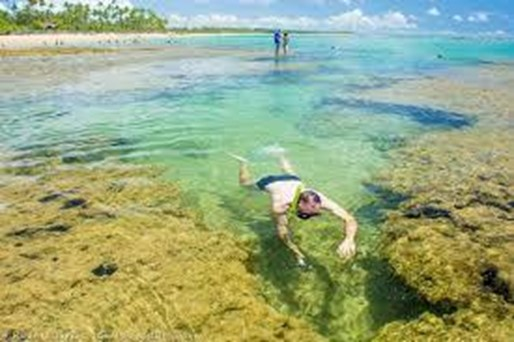
\includegraphics[width=.6\linewidth]{trigonometricas117}
\caption{Fonte: \href{guiaviagensbrasil.com}{Guia Viagens Brasil.com}}
\label{}
\end{figure}

É necessário pegar a maré com o nível mais baixo para curtir o mergulho com as maravilhas do mar. (\url{https://www.viajenaviagem.com/2013/04/como-usar-tabua-mares/})

\begin{figure}[H]
\centering

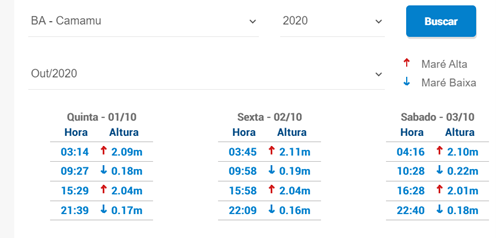
\includegraphics[width=.7\linewidth]{trigonometricas118}
\caption{Fonte: \href{https://www.climatempo.com.br/tabua-de-mares}{Climatempo}}
\label{}
\end{figure}

Assumindo que o comportamento periódico das marés seja definido por uma senóide da forma $y = a\cdot\sen(bx+c) + d$, encontre um modelo apenas usando os dados acima. Assuma também que o ponto mais alto assumido pela maré na semana das medições foi $2{,}11$ m e o mais baixo, $0{,}16$ m. Utilize o modelo para realizar uma previsão sobre os horários do dia de domingo, 04/10 onde a maré atingirá o ponto mais baixo e o mais alto. Quais os melhores horários para praticar snorkel naquele dia?

\ifdefined\prof
\begin{solucao}

\begin{itemize}
\item $a=0{,}98; b=0{,}52; c=0; d=1{,}14$
\item Horários de maré alta: $3{:}00$ e $15{:}00$
\item Horários de maré baixa $9{:}00$ e $21{:}00$
\item Melhores horários para o mergulho: $9{:}00$ e $21{:}00$
\end{itemize}
\end{solucao}
\fi

\end{document}